\documentclass[
    % draft,          % 草稿模式
    aspectratio=169,  % 使用 16:9 比例
]{ctexbeamer}
\mode<presentation>

\usetheme[min,light,blue]{sjtubeamer}
% 使用 maxplus/max/min 切换标题页样式
% 使用 red/blue 切换主色调
% 使用 light/dark 切换亮/暗色模式
% 使用外样式关键词以获得不同的边栏样式
%   miniframes infolines  sidebar* 
%   default    smoothbars split	 
%   shadow     tree       smoothtree

% \tikzexternalize[prefix=build/]
% 如果您需要缓存 tikz 图像,请取消注释上一行,并在编译选项中添加 -shell-escape。

\usepackage[backend=biber,style=gb7714-2015]{biblatex}
\addbibresource{thesis.bib}

%\institute[SJTUG]{上海交通大学 Linux 用户组} % 组织

\title{KASLR in the age of MicroVMs}
\subtitle{EuroSys 2022}       % 副标题
\author{Benjamin Holmes, Jason Waterman, Dan Williams}% 作者
\date{\today}                        % 日期  

\begin{document}

\maketitle                           % 创建标题页

\part{Outline}

\begin{frame}
  \frametitle{Outline}

microVM很关注启动速度,因此microVM通常省略bootstrap步骤,直接进入虚拟机kernel中启动,但是这使得vm缺少了KASLR的保护。

\vspace{0.15\textheight}

这篇文章分析了为什么不能够在bootloader过程中实现KASLR,并且将KASLR的功能实现在monitor中,取得了能够接受的性能开销。

\end{frame}

\part{Background}

\begin{frame}
  \frametitle{microVMs}
  microVMs: 常用于serverless中,运行时间短,必须能够快速启动。之所以是vm而不是container是因为vm的安全性更高。
\end{frame}

\begin{frame}
  \frametitle{Booting a microVM}
  \framesubtitle{通过bootloader启动bzImage}

  \begin{figure}
  	\centering
  	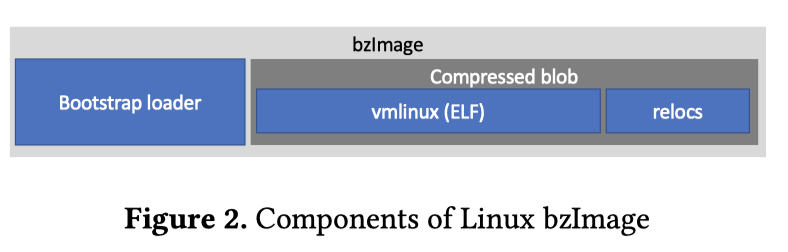
\includegraphics[width=0.8\textwidth]{img/bzImage.png}
  \end{figure}

%  kernel启动的经典格式是bzImage, bzImage有三个部分,第一个部分用于bootloader, bootloader的主要作用是对kernel elf文件进行解压缩与重定位,第二个部分是vmlinux保存kernel的可执行文件,第三部分与重定位有关,relocs里的每一项都代表一个需要重定位(R\_X86\_64\_32)的符号,它会指向一个物理地址,bootloader需要将重定位后的虚拟地址填入其中。
%
%  Bootloader有一个自己的stack和heap, bootloader首先要做的是将kernel的可执行文件解压并放在内存中,然后解析ELF文件,将每一段都放在指定内存中,这个指定内存与KASLR中的随机地址有关。
\end{frame}

\begin{frame}
  \frametitle{Booting a microVM}
  \framesubtitle{kernel直接启动}

  Modern的VM monitors(Fire-cracker, Cloud Hypervisor, QEMU)都支持跳过bootstrap直接启动一个未被压缩的kernel,而不是bzImage。

直接启动vm的kernel将不能够给vm实现KASLR。
\end{frame}

\begin{frame}
  \frametitle{KASLR}
  KASLR是对在kernel启动的时候对整个kernel做一个基地址随机化, 来抵抗ROP攻击。

  KASLR的两个主要问题不再是问题:
  \begin{itemize}
    \item KASLR在kernel运行过程中只进行一次(启动时)随机化: microVMs本身运行时间很短
    \item KASLR 粒度太大,一旦发生了内核地址泄漏,整个内核的KASLR就相当于无用: kptr\_restrict, FGKASLR
  \end{itemize}
\end{frame}

\begin{frame}
  \frametitle{Bring back KASLR to microVM}

  KASLR作为防止OS受到攻击的关键措施之一,并且自身的很多问题得到解决,所以作者强调KASLR还是有用武之地的。
  作者认为应该为microVM实现KASLR。

\end{frame}

\part{Contribution}

\begin{frame}
  \frametitle{Contribution 1: 指出microVM缺少KASLR}
  microVM缺少KASLR的保护,作者指出了这一点,并说这是他们的贡献之一。
\end{frame}

\begin{frame}
  \frametitle{Contribution 2: 分析了为什么不能够在bootstrap中实现KASLR}
  由于bootstrap启动的bzImage是压缩的,而direct boot的kernel image是未经过压缩的,作者首先研究compress对于microVM kernel启动时间的影响。
\end{frame}

\begin{frame}
  
  \begin{figure}
  	\centering
  	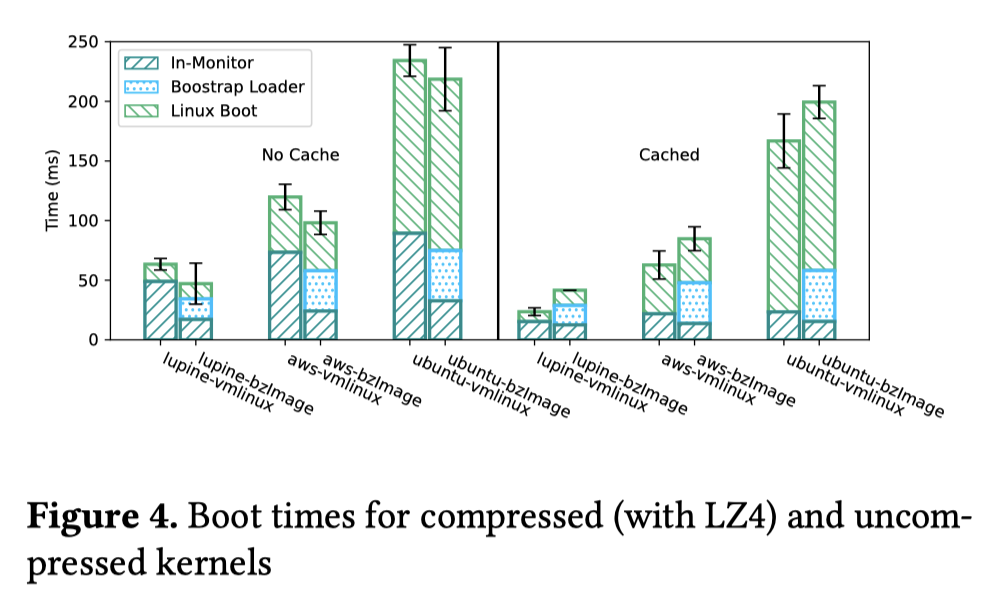
\includegraphics[width=0.6\textwidth]{img/boot_time_compare.png}
  \end{figure}

\begin{block}{实验1}
  分析有无cache的情况下,bootloader boot 和 direct boot哪个更快
\end{block}

%在没有cache的情况下,bootloader比dreict boot的启动速度要快,在有cache的情况下则相反。

\end{frame}

\begin{frame}
  \begin{figure}
  	\centering
  	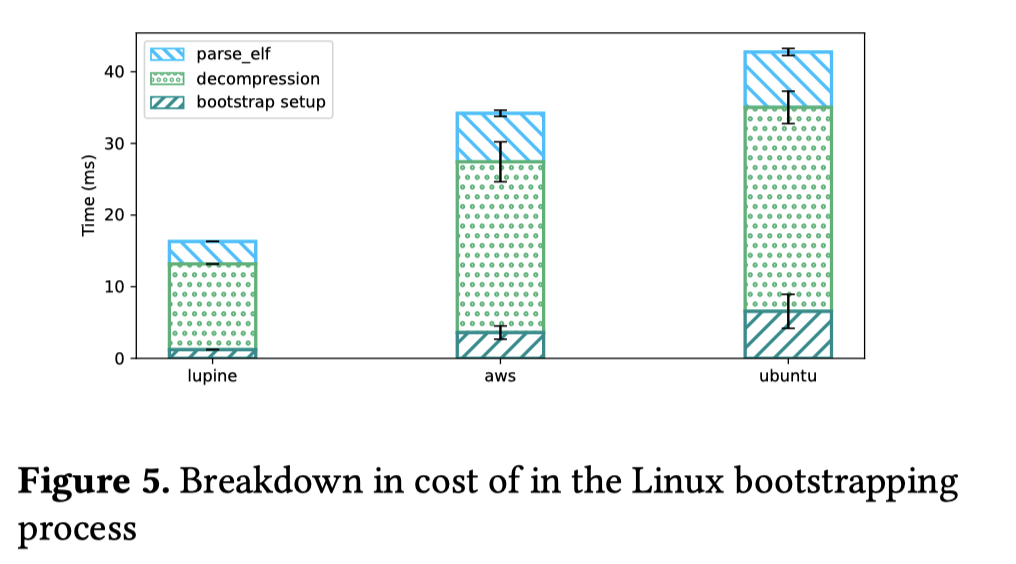
\includegraphics[width=0.6\textwidth]{img/boot_breakdown.png}
  \end{figure}

\begin{block}{实验2}
  分析bootloader中时间花在了哪些步骤
\end{block}

\end{frame}

\begin{frame}

既然bootloader中的主要时间是花在了解压缩上,而bootloader又是现阶段KASLR基于的工具,那一个直接的想法就是bootloader不需要解压缩,直接load一个uncompressed kernel,进行地址随机化就行。这样启动时间就会比bzImage好很多,事实上是否如此呢?

\end{frame}

\begin{frame}

  \begin{figure}
  	\centering
  	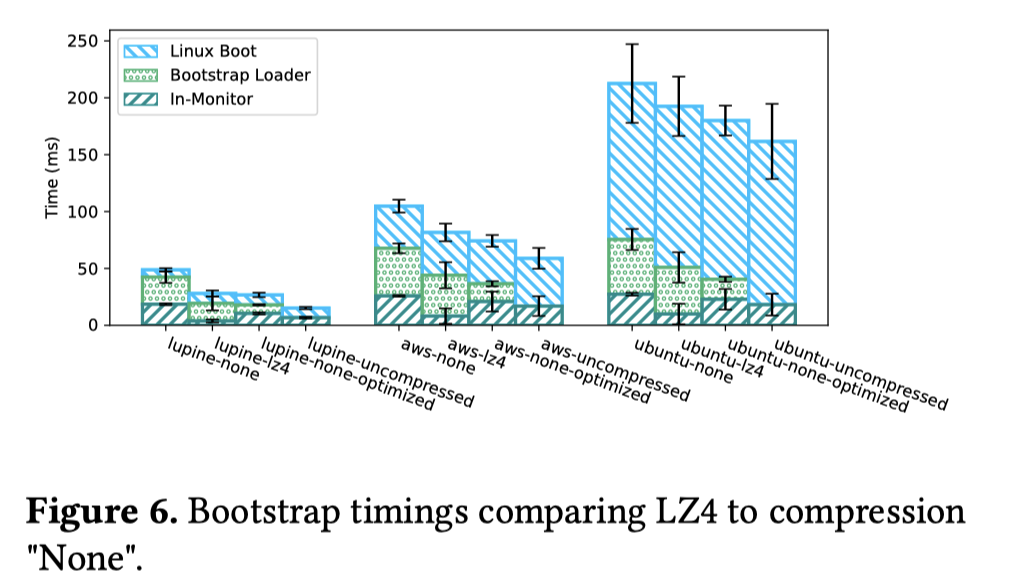
\includegraphics[width=0.55\textwidth]{img/no_compress.png}
  \end{figure}
  
\begin{block}{实验3}
  bootloader加载未经过压缩的kernel(不解压,直接copy)
\end{block}

性能甚至比加载压缩的kernel还要差, 作者修改了bootloader后,跳过了两次多余的image 拷贝后,再次测试:
%作者对此做了一个实验,由于bootloader不支持未压缩的bzImage, 
%作者使用了一个假装compressed的bzImage(实际上没有压缩),在解压缩的时候直接copy就好。
%然后作者发现,这种情况下性能仍然很糟糕,比有压缩的情况下性能还要糟糕。这是由于启动的时候,仍然需要:
%1) copy bzImage到gust memory里面,跳转到bootloader, 这时候的IO开销大于compressed的
%2) 将uncompressed kernel拷贝到一个另外的地址里 
%3) 做一次啥事都没干的"解压缩",然后再把"解压缩"后的内核代码拷贝到具体的物理内存地址里面。
%4) 跳转到解压后的起始地址。
%作者说这里的2) 3)两步是不需要的
\end{frame}

\begin{frame}
  \begin{figure}
  	\centering
  	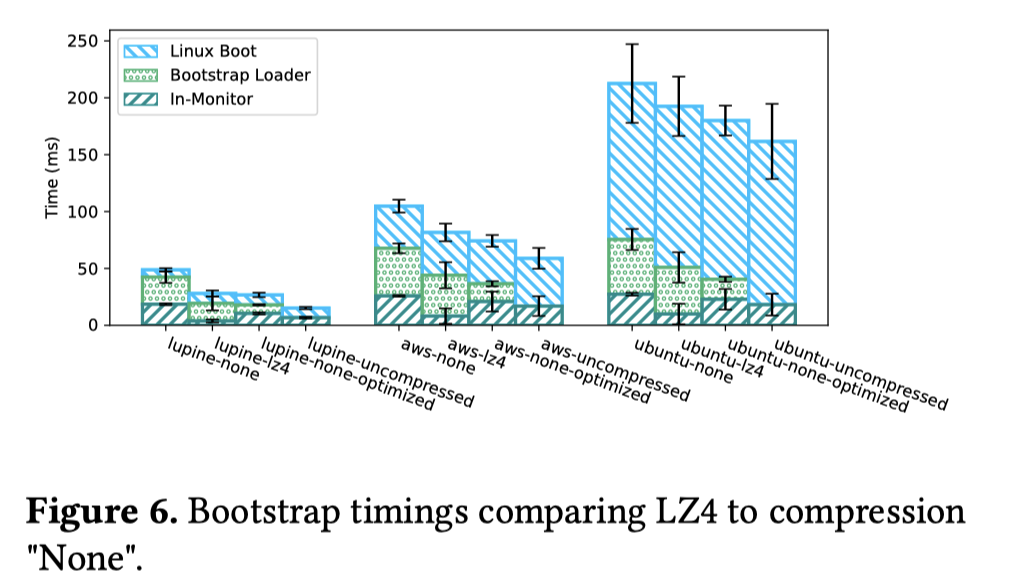
\includegraphics[width=0.55\textwidth]{img/no_compress.png}
  \end{figure}
\begin{block}{实验4}
  优化bootloader后的启动时间
\end{block}
  none-optimized依旧比uncompressed要慢许多,因此作者认为bootloader中实现KASLR是不可行的。于是引入了他们的设计in-monitor KASLR。
\end{frame}

\begin{frame}
  \frametitle{Contribution 3: 提出了在monitor中为vm实现KASLR的设计,并在Firecracker中实现}
核心的设计是在monitor中完成原来在bootloader中完成的parse ELF和重定位这两个事情。然后直接跳转到guest kernel中运行。
\end{frame}

\begin{frame}
  \begin{figure}
  	\centering
  	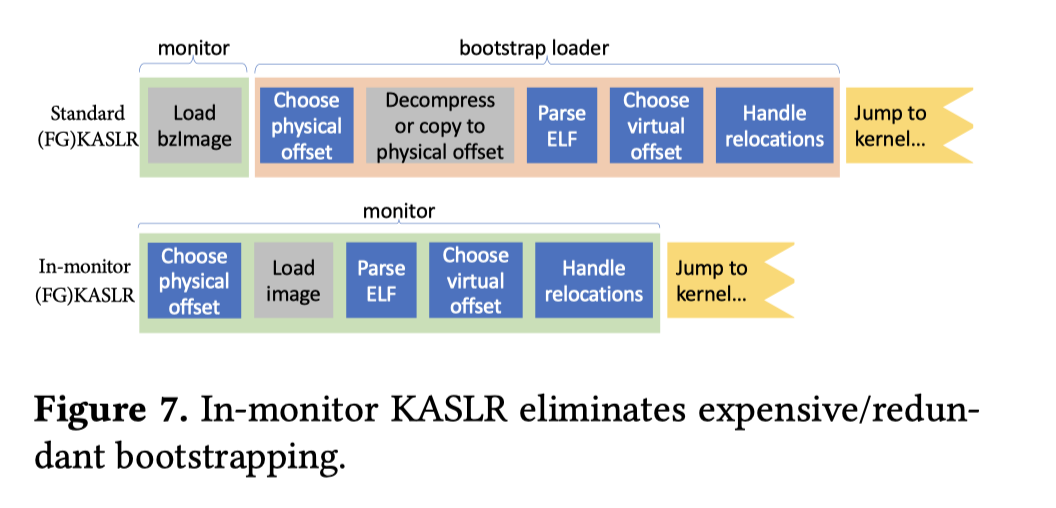
\includegraphics[width=0.6\textwidth]{img/in_monitor.png}
  \end{figure}
  相当于除了解压缩其他bootloader做的事情都在monitor中完成
\end{frame}

\begin{frame}
  \begin{figure}
  	\centering
  	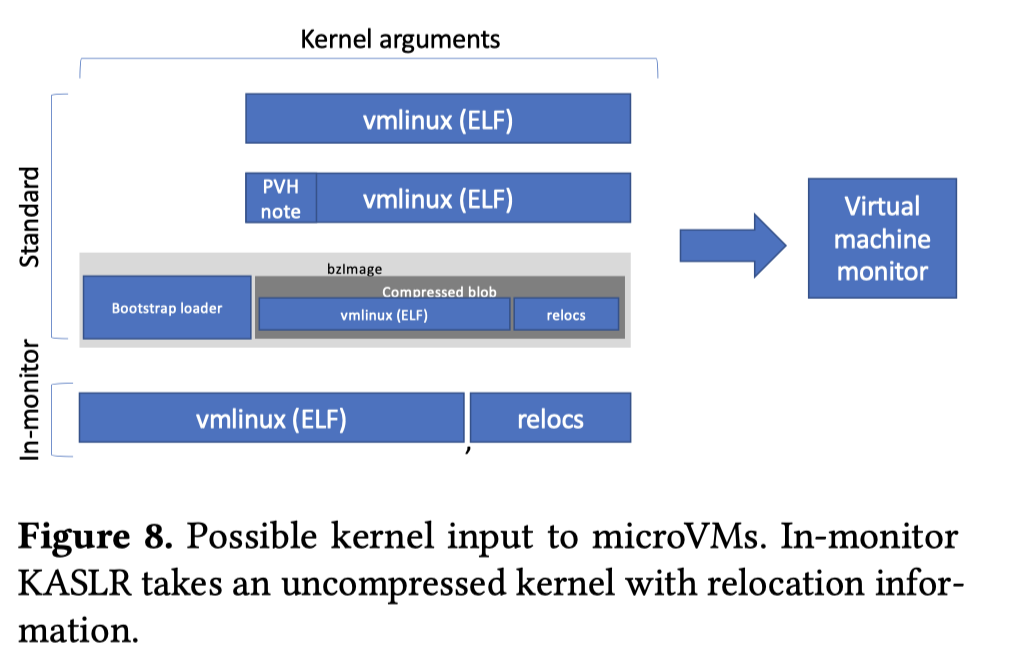
\includegraphics[width=0.6\textwidth]{img/kernel_input.png}
  \end{figure}
  为了完成relocation需要额外的input信息(bzImage里面的relocs)
\end{frame}

\part{Implementation}

\begin{frame}
  \frametitle{实现}

在Fire-cracker v0.26中实现了in-monitor的KASLR与FGKASLR。

KASLR 不超过200行,FGKASLR不超过1000行。

简要介绍下实现上的一些点:

  \begin{itemize}
    \item 重定位后不立刻更新/proc/kallsyms,ORC stack unwinder table(用于stacktrace)。因为micro-VMs的应用程序其实不会访问它。
    \item vmlinux.relocs由kernel build 程序直接生成,monitor直接读就好
    \item 直接使用Rust语言提供的随机数
    \item hardcode 内核启动参数 (实现还不完备)
  \end{itemize}

\end{frame}


\part{Evaluation}

\begin{frame}
\begin{figure}
	\centering
	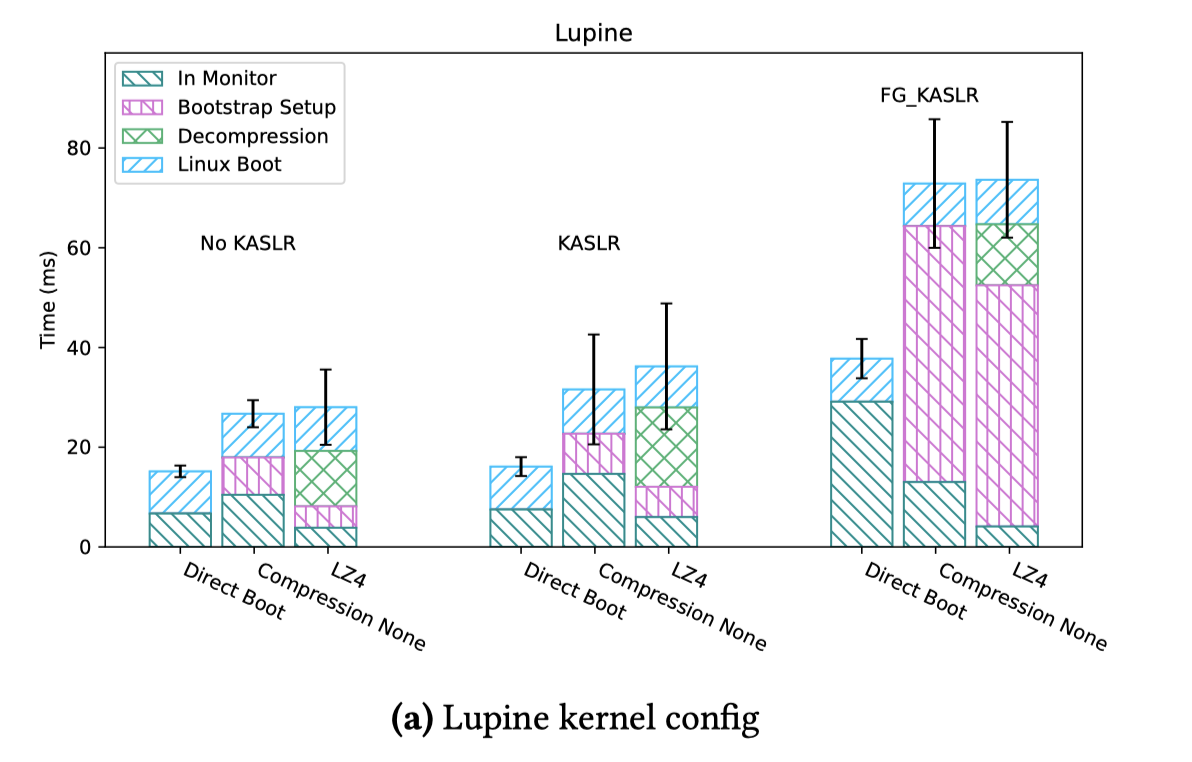
\includegraphics[width=0.65\textwidth]{img/lupin_eval.png}
  \caption{lupine kernel 代表single-purpose很小的kernel config,用于unikernel-based environments}
\end{figure}

\end{frame}

\begin{frame}
\begin{figure}
	\centering
	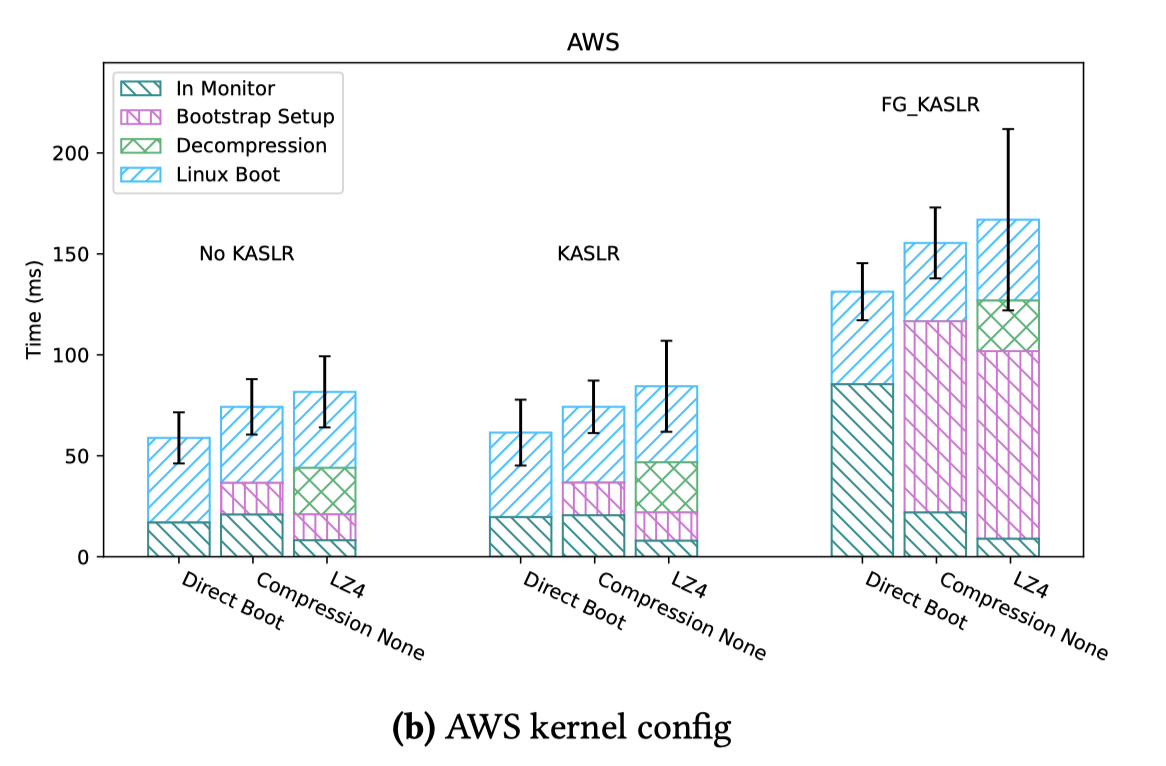
\includegraphics[width=0.65\textwidth]{img/aws_eval.png}
  \caption{AWS kernel指FireCracker上vm用的kernel config,代表micro-vm的配置}
\end{figure}

\end{frame}


\begin{frame}
\begin{figure}
	\centering
	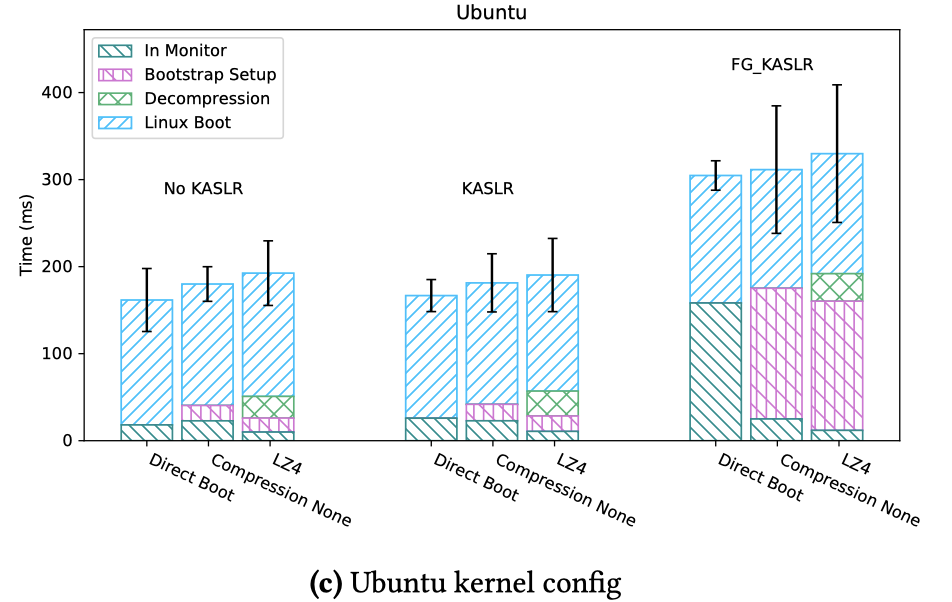
\includegraphics[width=0.5\textwidth]{img/ubuntu_eval.png}
  \caption{ Ubuntu是Ubuntu 18.04的config, 代表kernel发行版的配置}
\end{figure}
in-monitor KASLR 相对于之前提到过的修改过的bootloader实现KASLR的方式比起来在Luping,AWS和Ubuntu分别有15ms, 13ms, 16ms的启动时间提升。相比于传统的bzImage boot则分别有20ms, 23ms, 25ms的启动时间提升。

\end{frame}

\begin{frame}

\begin{figure}
	\centering
	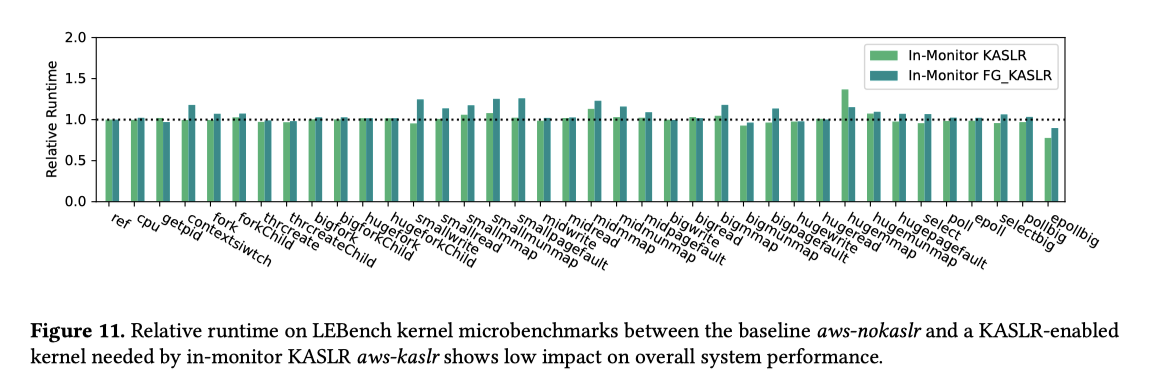
\includegraphics[width=0.7\textwidth]{img/lebench.png}
\end{figure}

通过in-monitor中实现KASLR对整体性能的overhead很小,通过LEBench microbenchmarks测试得出KALSR仅有不到1\%的运行时间影响,FGKASLR会慢上大约7\%。

\end{frame}

\part{Discussion}

\begin{frame}
当前的工作是建立在有cache的情况下未压缩的kernel image比bzImage启动更快的前提下,但是在unikernel的情况下,每个app对应一个kernel,这时候没有足够的cache缓存kernel image。这可能导致这种情况下重新在bootloader实现KASLR更佳
\end{frame}

\part{Conclusion}

\begin{frame}
  \frametitle{总结}
  \begin{itemize}
    \item 为microVM在monitor中实现了(FG)KASLR
    \item 在monitor中实现KASLR是一个非常直接的想法
    \item 在monitor中KASLR实现是一个比较工程的问题
    \item 论文也并没有表现出它们有哪些创新的设计,反而将很大的篇幅介绍背景,motivation和测试步骤。
  \end{itemize}
\end{frame}

%\begin{frame}
%\begin{itemize}
%  \item FGKASLR现在的应用情况: 在Linux 5.11版本上被研究者提出, 但是还没有合并进入主线。
%  \item 这个工作基于的FireCracker基于的版本是0.26,说明这篇工作差不多是去年eurosys前两个月做的。
%  \item ORC stack uninwder table 是什么: Fixing the bug requires that developers understand the state of your machine at the time of the crash. One of the most critical clues for debugging is the stacktrace, produced by the kernel’s stack unwinder. But the kernel’s unwinders are not reliable 100\% all of the time. The x86 ORC unwinder patch series, posted to the Linux kernel mailing list by Josh Poimboeuf, aims to change that.
%  \item relocs的作用
%  \item direct boot 为什么不需要relocation? 可能qemu已经做过了,但是如果qemu帮助做relocation,帮助实现KASLR不是顺理成章的事情吗?那这篇论文的贡献在哪里? direct boot是不做relocation
%  \item none-optimized和in-monitor的性能比较
%  \item 如果不做KASLR还需要relocation吗 应该是不需要的,因为要做relocation就需要有relocs,但是按照论文的意思是relocs是他们新增加的,之前firecracker并不会读relocs文件
%\end{itemize}
%\end{frame}

\makebottom       % 创建结束页

\end{document}
